\subsection{平行线}\label{subsec:czjh1-2-4}

笔直的两条铁轨(图 \ref{fig:czjh1-2-13})、黑板相对的两边,都给我们以平行线的形象。
如果画出它们的图形,都是在同一平面内的两条线段(图 \ref{fig:czjh1-2-14})。
我们把这样的两条线段都向两方延长,它们总不会相交。这就是说,
在同一个平面内,两条直线除相交的情形外,还有不相交的情形。

\begin{figure}[htbp]
    \centering
    \begin{minipage}[b]{7cm}
        \centering
        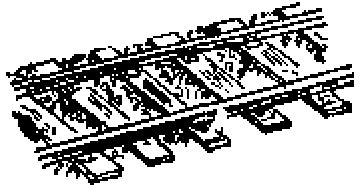
\includegraphics[width=5cm]{../pic/czjh1-ch2-13.png}
        \caption{}\label{fig:czjh1-2-13}
    \end{minipage}
    \qquad
    \begin{minipage}[b]{7cm}
        \centering
        \begin{tikzpicture}
    \tkzDefPoints{0/0/A, 2/0.5/B, 0/-1.0/C, 2/-0.5/D}

    \tkzDrawLines[add=0.3 and 0.3](A,B  C,D)
    \tkzLabelPoints[above](A, B, C, D)
\end{tikzpicture}


        \caption{}\label{fig:czjh1-2-14}
    \end{minipage}
\end{figure}

在同一个平面内不相交的两条直线叫做\zhongdian{平行线}。

平行用符号“$\pingxing$”表示。如图 \ref{fig:czjh1-2-14},直线 $AB$ 和 $CD$ 是平行线,
记作 “$AB \pingxing CD$”, 读作 “$AB$ 平行于 $CD$”。

在同一个平面内,两条直线的位置关系只有两种:平行或相交。

直线 $AB$ 可以看作是 $AB$ 上所有的点的集合,直线 $CD$ 可以看作是 $CD$ 上所有的点的集合。
直线 $AB$ 和 $CD$ 相交,就是这两个集合有一个并且只有一个公共元素(它们的交点)。
直线 $AB$ 和 $CD$ 平行,就是这两个集合没有公共元素。

\begin{lianxi}
    举出几个平行线的实例。
\end{lianxi}


